\ifx\wholebook\relax \else

\documentclass[b5paper]{article}
\usepackage[nomarginpar
  %, margin=.5in
]{geometry}

\addtolength{\oddsidemargin}{-0.05in}
\addtolength{\evensidemargin}{-0.05in}
\addtolength{\textwidth}{0.1in}

\usepackage[en]{../prelude}

\setcounter{page}{1}

\begin{document}

\title{Numerals}

\author{Xinyu LIU
\thanks{{\bfseries Xinyu LIU} \newline
  Email: liuxinyu99@hotmail.com \newline}
  }

\maketitle
\fi

\markboth{Numerals}{A tour of numbers}

\ifx\wholebook\relax
\chapter{Numerals}
\fi

\epigraph{The total number of minds in the universe is one.}{Erwin Schrödinger}

Numbers appear everywhere in our daily life. For example, this news: \enquote{\textit{The 2024 Paris Olympic Games to an end on Sunday August 11, 2024. Paris is the second city, after London, to host the Summer Olympics three times. It set a record of gender equality, with 5,250 male and 5250 female athletes. In total, 32 sports and 329 events were featured, with 206 countries and regions participating. Four new sports made their debut: skateboarding, surfing, sport climbing, and breakdancing. A total of 329 gold medals were up for grabs. Athletes from various countries and regions demonstrated outstanding athleticism. The United States and China tied for the most gold medals, with each securing 40. The United States also led in silver medals with 44 and bronze medals with 42.}} It contains 14 numbers among the total of 120 words. We don't know who invented the numerals because they show up in almost all historic documents to the very early time. Some believe numerals arose with language. Anthropologists identified numbers inscribed in bones, stones, caves, clay, etc. We can also find such clues in our languages, for example in English, eleven comes from `endleofan', meaning (ten) left one; twelve comes from `twelf', meaning left two.

\section{Rosetta stone}
\index{Rosetta stone}

\begin{figure}[htbp]
 \centering
 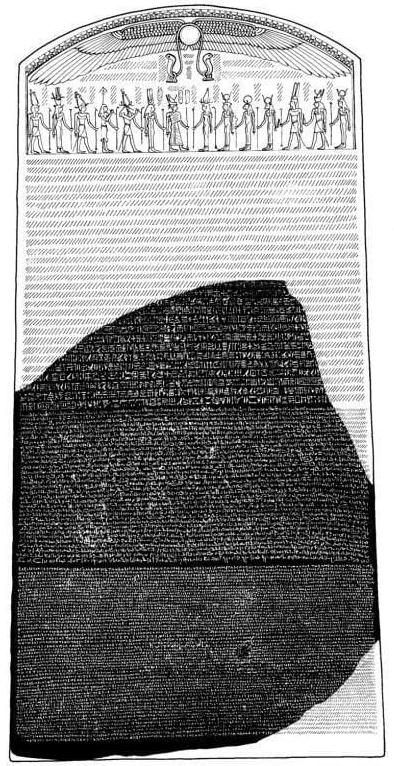
\includegraphics[scale=0.5]{img/Rosetta-stone-recons}
 \caption{Rosetta stone was broken in the middle.}
 \label{fig:rosetta-stone-recons}
\end{figure}

There is a famous object in room 4, the British museum. It's the Rosetta stone, a broken inscribed stela with the length of 112cm, the width of 76cm (\cref{fig:rosetta-stone-recons}). One can identifies some Greek characters like \cref{fig:rosetta-greek} (see \cref{tab:greek-alphabet} of Greek alphabet) in the bottom, while the remaining are mystery ancient characters. When read them carefully, there are two different types: a curved form as in \cref{fig:rosetta-demotic} in the middle of the stone, and some small pictures as in \cref{fig:rosetta-hieroglyphs} on the top.

\begin{figure}[htbp]
  \centering
  \subcaptionbox{54 lines in Ancient Greek.\label{fig:rosetta-greek}}{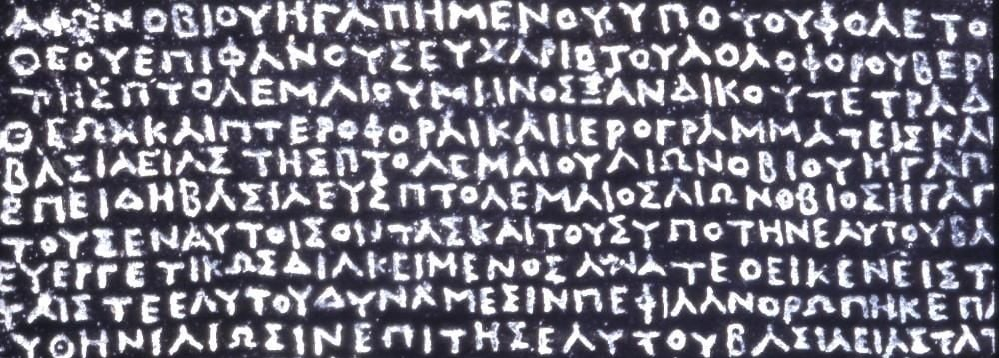
\includegraphics[scale=0.5]{img/Rosetta-Greek}} \\
  \subcaptionbox{32 lines in Demotic, a cursive form of Hieroglyphics use for ordinary document.\label{fig:rosetta-demotic}}{\quad 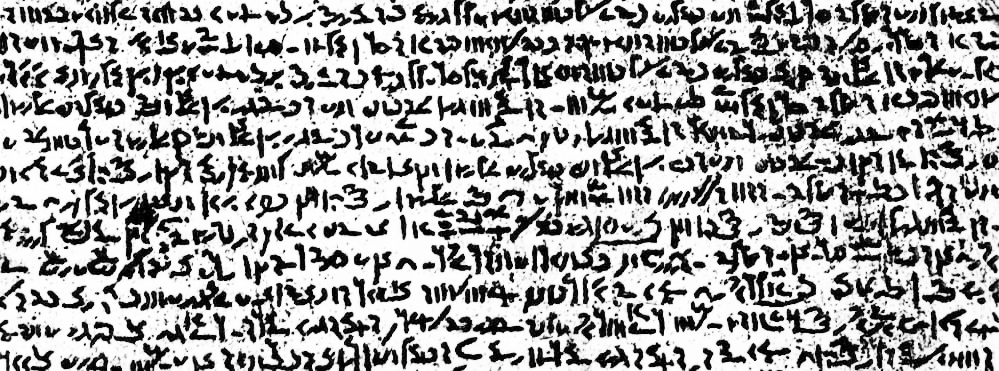
\includegraphics[scale=0.5]{img/Rosetta-Demotic}\quad} \\
  \subcaptionbox{14 lines in Hieroglyphic, the script most used for religious texts.\label{fig:rosetta-hieroglyphs}}{\qquad 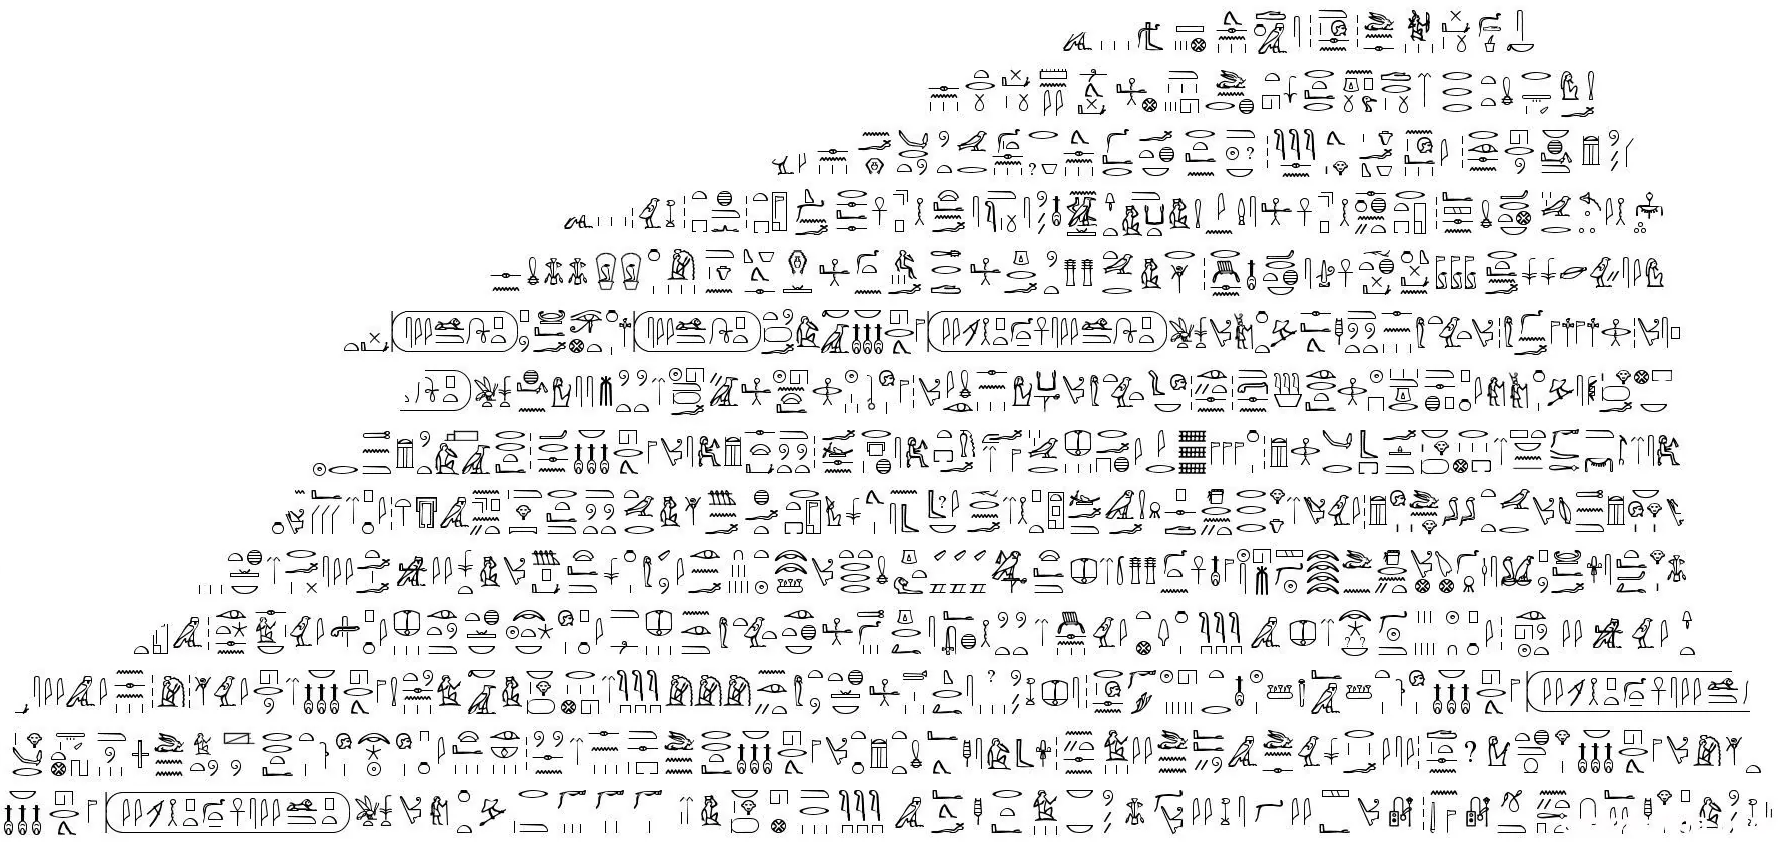
\includegraphics[scale=0.3]{img/Rosetta-Hieroglyphs-c}\qquad}
  \caption{Three different scripts and languages on Rosetta stone.}
  \label{fig:rosetta-stone}
 \end{figure}

The discovery of the Rosetta stone was during the Expedition when Napoleon Bonaparte campaigned in Egypt from 1798 to 1701. The troop had about 3,800 soldiers, a fleet of 326 ships, and 167 most distinguished scientists and scholars directed by mathematician Gaspard Monge\cite{Harrison-2023}. This gave the expedition a scientific purpose, aiming to conduct research and show off scientific advances. The fleet secretly departed from Toulon, and lucky by-passed the British Royal Navy in thick fog. Napolean's army captured Alexandria on 2 July.

\ifx\wholebook\relax \else
\section{Answer}
\shipoutAnswer

 \begin{table}[htbp]
     \centering
     \begin{tabular}{|c|c|c||c|c|c|}
         \hline
               \textbf{Upper} & \textbf{Lower} & \textbf{Pronunciation} & \textbf{Upper} & \textbf{Lower} & \textbf{Pronunciation} \\
         \hline
         A         & $\alpha$    & Alpha &      N         & $\nu$         & Nu \\
         B         & $\beta$     & Beta &       $\Xi$         & $\xi$         & Xi \\
         $\Gamma$  & $\gamma$    & Gamma &      O    & o    & Omicron \\
         $\Delta$  & $\delta$    & Delta &      $\Pi$         & $\pi$         & Pi \\
         E         & $\epsilon$  & Epsilon &    P        & $\rho$        & Rho \\
         Z         & $\zeta$     & Zeta &       $\Sigma$      & $\sigma$      & Sigma \\
         H         & $\eta$      & Eta &        T        & $\tau$        & Tau \\
         $\Theta$  & $\theta$    & Theta &      Y    & $\upsilon$    & Upsilon \\
         I         & $\iota$     & Iota &       $\Phi$        & $\phi$        & Phi \\
         K         & $\kappa$    & Kappa &      X        & $\chi$        & Chi \\
         $\Lambda$ & $\lambda$   & Lambda &     $\Psi$        & $\psi$        & Psi \\
         M         & $\mu$       & Mu &         $\Omega$      & $\omega$      & Omega \\
         \hline
     \end{tabular}
     \caption{Greek alphabet}
     \label{tab:greek-alphabet}
 \end{table}

\begin{thebibliography}{99}

\bibitem{Harrison-2023}
Mark W. Harrison. ``Napoleon's Campaign in Egypt and Syria''. World History Encyclopedia, 27 April, 2023, \url{https://www.worldhistory.org/Napoleon's_Campaign_in_Egypt_and_Syria/}. Accessed 26 February 2025.

%% \bibitem{wiki-number}
%% Wikipedia. ``History of ancient numeral systems''. \url{https://en.wikipedia.org/wiki/History_of_ancient_numeral_systems}

%% \bibitem{Calvin-Clawson-1994}
%% Calvin C Clawson. ``The Mathematical Traveler, Exploring the Grand History of Numbers''. Springer. 1994, ISBN: 9780306446450

%% \bibitem{wiki-babylonian-num}
%% Wikipedia. ``Babylonian numerals''. \url{https://en.wikipedia.org/wiki/Babylonian_numerals}

\end{thebibliography}

\expandafter\enddocument
%\end{document}

\fi
